% pdflatex notes.tex 

\documentclass[twocolumn]{article}
\usepackage{amsfonts}
\usepackage{pifont}
\usepackage{hyperref}
\usepackage{tikz}
\usetikzlibrary{bayesnet}
\usepackage{amsmath}
\usepackage{amssymb}

\begin{document}

\title{Notes on \href{https://arxiv.org/pdf/2203.11618.pdf}{Distributing Collaborative Multi-Robot Planning with Gaussian Belief Propagation}}
%\description{wassup}
\author{Rom Parnichkun}

\maketitle

\section{Factor Graphs}

A joint probability distribution $p(V)$ is factorised with a factor graph as:
\begin{equation}
    p(V) = \prod_{j}^{N_f}{f_j(V_j)},
\end{equation}
where given a set of variables $V = {v_i}_{i=1:N_v}$, a factor node $f_j$ is connected to a subset of the variables, $V_j \subseteq V$, and $N_v$ is the number of variables.

\begin{figure}[h]
\centering
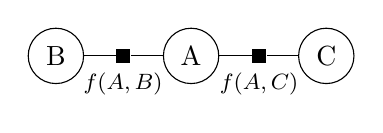
\begin{tikzpicture}

  % Define nodes
  \node[latent]                               (a) {A};
  \node[latent, left=of a]     (b) {B};
  \node[latent, right=of a]    (c) {C};
  \factor[left=of a, right=of b] {a-b} {below:$f(A,B)$} {a,b} {} ; %
  \factor[right=of a, left=of c] {a-c} {below:$f(A,C)$} {a,c} {} ; %

\end{tikzpicture}
\caption{An example of a factor graph.}
\end{figure}

Solvers such as \href{https://gtsam.org/get_started/}{GTSAM} exploit the sparsity revealed by the factor graph for efficient maximum a-posteriori (MAP) inference using sparse linear algebra, and such algorithms are efficient for centralised solvers which have full access to the graph.

\section{Gaussian Belief Propagation}

GBP is an alternative method to perform inference on a factor graph. It is a subclass of belief propagation which operate using node-wise local computation and message passing, enabling distributed solutions.

The canonical form of a Gaussian distribution is used.
\begin{equation}
\mathcal{N}(x; \mu,\Sigma) = \mathcal{N}(x; \eta,\Lambda),
\end{equation}
in which $\Lambda = \Sigma^{-1}$ and $\eta = \Sigma^{-1}\mu$. 
In GBP, variables $V$ are assumed to be Gaussian; thus each variable has a belief $b(v_i) = \mathcal{N}^{-1}(v_i;\eta_i,\Lambda_i)$. Factors $F = {f_i}_{i=1:N_f}$ are a probabilistic Gaussian constraint between variables. $f_i(V_j)$ is an arbitrary function that connects variables $V_j$, and it may be non-linear.  
\subsection{Variable Belief Update}
\begin{equation}
    b(v_i) = \prod_{f\in n(v_i)}{m_{f \rightarrow i}(v_i)},
\end{equation}

where $n(v_i) \subseteq F$ is the set of factors that the variable $v_i$ is connected to, and $m_{f \rightarrow i}(v_i) = \mathcal{N}^{-1}(v_i; \eta_{f \rightarrow i},\Lambda_{f \rightarrow i})$ is the message from a factor to the variable. As we are using the canonical form, the product between distributions can be rewritten as a summation:
\begin{equation}
    \eta_i = \sum_{f_\in n(v_i)}{\eta_{f \rightarrow i}},
\end{equation}
\begin{equation}
    \Lambda = \sum_{f_\in n(v_i)}{\Lambda_{f \rightarrow i}}.
\end{equation}

\subsection{Variable to Factor Message}
\begin{equation}
    m_{v_i \rightarrow j}(f_j) = \prod_{f \in n(v_i) \setminus f_j}{m_{f \rightarrow i}(v_i)}.
\end{equation}

\subsection{Factor Likelihood Update}
The likelihood of factor $f(V_j)$ with measurement function $h(V_j)$, observation $z_s$, and precision of the observation $\Lambda_s$, can be expressed as a Gaussian distribution $\mathcal{N}^{-1}(V_j; \eta_f, \Lambda_f)$, where $\eta_f = \Lambda_s(z_s - h(V_j))$ and $\Lambda_f = \Lambda_s$. This however only holds if $h(V_j)$ is linear. In the non-linear case, we linearise using first-order Taylor expansion: $h(V_j) = h(V^0_j) + J(V_j - V^0_j)$.
\begin{equation}
    \eta_{f} = J^T\Lambda_m(JV^0_j+z_m-h(V^0_j)),
\end{equation}
\begin{equation}
    \Lambda{f} = J^T\Lambda_mJ,
\end{equation}
where $V^0_j$ is the linearisation point, the current state of the variables. In this work $z_m = 0$ for all factors, meaning that the factor energy is purely a function of the states.

\subsection{Factor to Variable Message}
\begin{equation}
    m_{f \rightarrow i}(v_I) = \sum_{v_j \in V_j \\ v_i}{f(V_j)}\prod_{v_j \in V_j \\ v_i}{m_{v_j \rightarrow f}(v_j)}.
\end{equation}

\section{Method}

\subsection{Modelling a robot moving through a 2D plane}

\begin{equation}
    \dot{x}_i = Ax_i + Bu_i + Fw_i,
\end{equation}
\begin{equation}
    A  = \begin{bmatrix}
        0 & 1\\
        0 & 0
    \end{bmatrix},
    B = 0,
    F = \begin{bmatrix}
        0\\1
    \end{bmatrix},
\end{equation}
where $w \sim \mathcal{N}(0, Q_d)$ is a white noise with covariance matrix $Q_d = \sigma^2_dI$.
$X_i$ represents the robot's position and velocity at that particular moment in time.
\begin{equation}
    X_i = \begin{bmatrix}
        x_i & y_i & \dot{x}_i & \dot{y}_i
    \end{bmatrix}^T.
\end{equation}
The trajector of the robot is represented by $N$ such states, from $X_0$ to $X_{N-1}$.
The optimal trajectory solution can be found by solving for the maximum a posteriori (MAP) solution $X^*$ for the trajectory states.

Nodes of the factor graph represents the robot states through time (see Figure \ref{fig:robot_states}).

\begin{figure}[h]
    \centering
    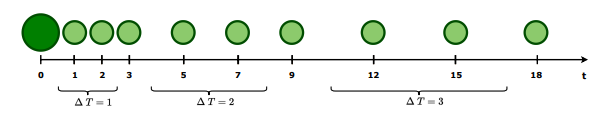
\includegraphics[width=3in]{figures/robot_states.png}
    \caption{Nodes represents the robot's state.}
    \label{fig:robot_states}
\end{figure}
\begin{figure}[h]
    \centering
    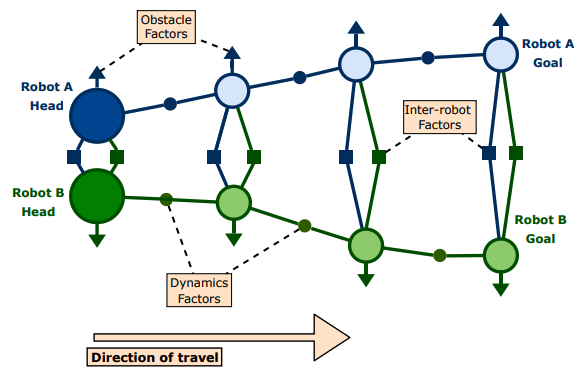
\includegraphics[width=3in]{figures/factor_graph.png}
    \caption{An example of the factor graph.}
    \label{fig:factor_graph_example}
\end{figure}

There are four types of factors that this study considers. 

\subsection{Pose Factor}

\begin{equation}
    h_p(X_i) = X_i,
\end{equation}
\begin{equation}
    \Sigma_p = \sigma^2_pI,
\end{equation}

\subsection{Dynamics Factor}

\begin{equation}
    h_d(X_i, X_{i+1}) = \Phi(t_{i+1}, t_i)X_i - X_{i+1},
\end{equation}
\begin{equation}
    \Sigma_d = \begin{bmatrix}
        \frac{1}{3}\Delta t^3_iQ_d & \frac{1}{2}\Delta t^2_i Q_d \\
        \frac{1}{2}\Delta t^2_iQ_d & t_i Q_d
    \end{bmatrix},
\end{equation}
where
\begin{equation}
    \Phi(t_b, t_a) = \begin{bmatrix}
        1 & (t_b - t_a)1 \\
        0 & 1
    \end{bmatrix}
\end{equation}
is the state-transition matrix from time $t_a$ to time $t_b$. This factor encourages a zero acceleration and therefore a feasible and smooth tarjectory.

\subsection{Obstacle Factor}

$h_O(X_i)$ is equal to 1 at or within the obstacle boundary and decreases exponentially to 0 at a distance of one robot radius away from the obstacle (kinda similar to a reward function).
The factor covariance is $\Sigma_O = \sigma_O I$.

\subsection{Inter-robot Factor}

The factor has a non-zero energy cost if the distance between the robots at a particular timestep is less than the critical distance distance $r^* = 2r_{robot} + \epsilon$ where $\epsilon$ is a small safety distance.
\begin{equation}
    g(p) = 
    \begin{cases}
        1-\frac{P}{r^*},& p \leq r^*\\
        0,              & \text{otherwise}
    \end{cases}.\footnote{This is known as a truncated hinge loss.}
\end{equation}
There is the possibility that robot tarjectories could interesect in between two consecutive timesteps. To avoid this issue we allow for K-opint linear interpolation between timesteps in the inter-robot factor.
\begin{equation}
    h_r(X_{A,i}, X_{B,i}) = [g(r_{i+\frac{k}{K}}] \rvert_{0 \leq k \leq K-1}.
\end{equation}
\begin{equation}
    \Sigma_r = \sigma_i I
\end{equation}
where $\sigma_i = \sigma_rt_i$.

\subsection{Goal State Update}

Goal state $X_{N-1}$ is updated as:
\begin{equation}
    X_{N-1} \leftarrow \begin{bmatrix}
        x_{N-1} + \tau v^*_{N-1} \\
        v^*
    \end{bmatrix},
\end{equation}
where
\begin{equation}
    \tau = \begin{cases}
        1 & ||x_{N-1} - x_0|| \leq r_{max}\\
        (\dot{x_0}\cdot v^*) & \text{otherwise}
    \end{cases}
\end{equation}
and $r_{max} = t_{N-1}||v^*||$.

\end{document}
